\documentclass[11pt]{report}
% packages
% Fran Burstall's Bath thesis package
\usepackage{baththesis}
\usepackage{amssymb} %for Blackboard bold etc \usepackage{graphicx} %for including eps graphics % front matter
\usepackage[pdftex]{graphicx}
\usepackage{url}

\title{ Nonlinear Fictional Analysis\\and Harmonic Maps In Eight Dimensional Phase Space} \author{Yongliang Yang}
%\degree{Doctor of Philosophy}
\degree{ Master of Science }
\department{Department of Computer Sciences} \degreemonthyear{January 2015}
\norestrictions

\begin{document}
\maketitle
\begin{abstract}
In this thesis numerous seminal results are proved which will decisively shape the future development of the subject. \end{abstract}


\chapter{Introduction}
\label{ch:intro}
This document is based on the Bath Thesis Package by Fran Burstall \cite{Burstall}.
Please note that the headings and text are just examples written in fun.  The important thing are formatting facilities available. I have demonstrated :
\begin{itemize}
\item Overall format of thesis
\item Headings including chapter, section, subsection
\item referring to figures, sections, chapters, tables (as in see this chapter~\ref{ch:intro}).
\item Citations and the bibliography list
\item Maths environment (and some variations)
\item Figures
\item Tables
\item Itemized lists such as this one (also try substituting itemize for enumerate).
\end{itemize}

The text below, the names of the chapters and sections will be decided between student and supervisor.


\section{The Problem}
\label{sec:problem}
\begin{figure}[htb]
  \centering
    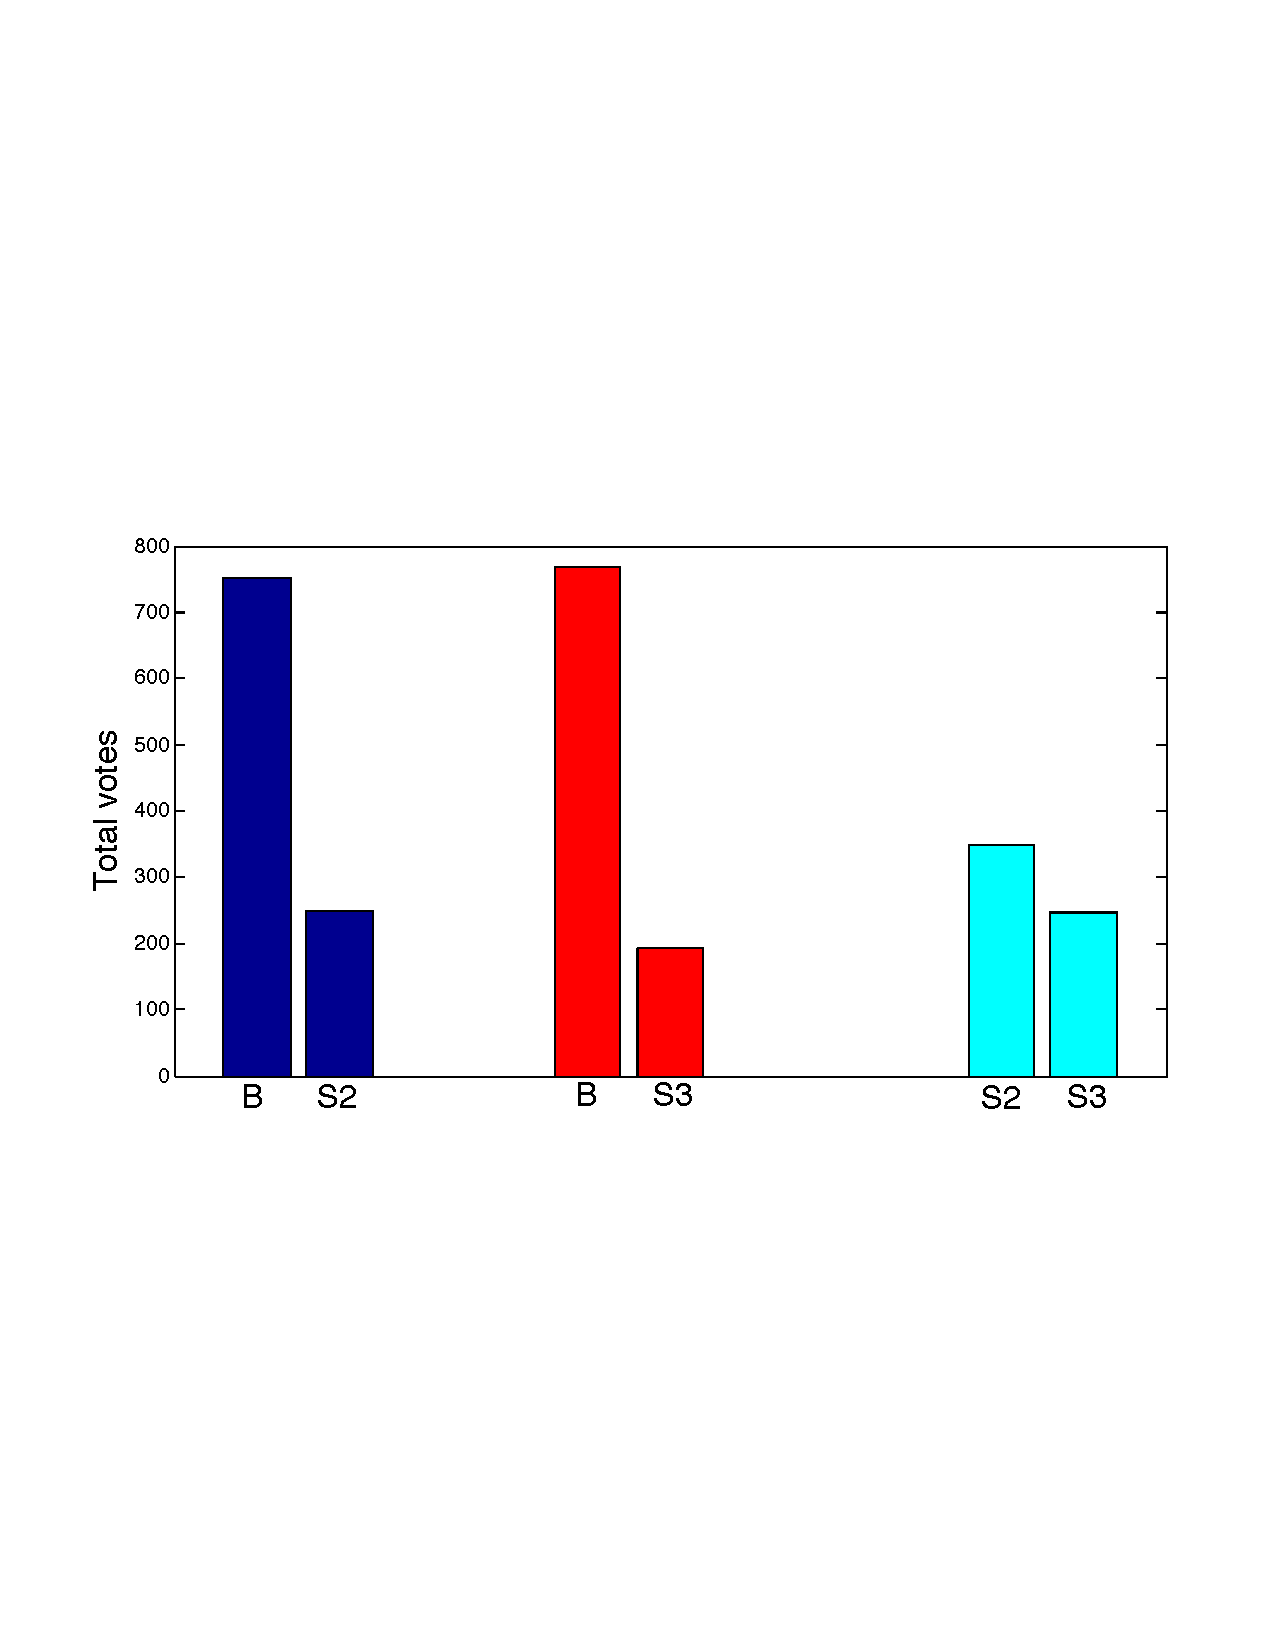
\includegraphics[width=.8\linewidth]{images/allComparison.pdf}
  \caption{\label{fig:all}
           An unrelated bar chart.}
\end{figure}

We begin by divulging the third secret of the Universe, namely that if I told you I would have to kill you.
This is not really illustrated by the irrelevant Figure~\ref{fig:all}
Grasping this fact enables us to move quickly into the next chapter.

\begin{figure}[htb]
  \centering
    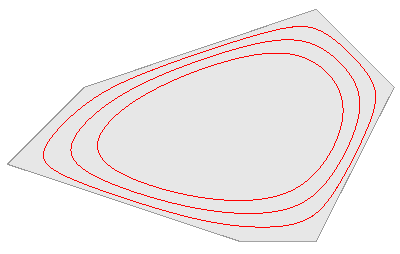
\includegraphics[width=.8\linewidth]{images/unweightedlog6.png}
  \caption{\label{fig:unweightedlog6}
           Three example curves.}
\end{figure}

Here is some gratuitous Latin. Lorem ipsum dolor sit amet, consectetur adipisicing elit, sed do eiusmod tempor incididunt ut labore et dolore magna aliqua. Ut enim ad minim veniam, quis nostrud exercitation ullamco laboris nisi ut aliquip ex ea commodo consequat. Duis aute irure dolor in reprehenderit in voluptate velit esse cillum dolore eu fugiat nulla pariatur. Excepteur sint occaecat cupidatat non proident, sunt in culpa qui officia deserunt mollit anim id est laborum. Lorem ipsum dolor sit amet, consectetur adipisicing elit, sed do eiusmod tempor incididunt ut labore et dolore magna aliqua. Ut enim ad minim veniam, quis nostrud exercitation ullamco laboris nisi ut aliquip ex ea commodo consequat. Duis aute irure dolor in reprehenderit in voluptate velit esse cillum dolore eu fugiat nulla pariatur. Excepteur sint occaecat cupidatat non proident, sunt in culpa qui officia deserunt mollit anim id est laborum. Lorem ipsum dolor sit amet, consectetur adipisicing elit, sed do eiusmod tempor incididunt ut labore et dolore magna aliqua. Ut enim ad minim veniam, quis nostrud exercitation ullamco laboris nisi ut aliquip ex ea commodo consequat. Duis aute irure dolor in reprehenderit in voluptate velit esse cillum dolore eu fugiat nulla pariatur. Excepteur sint occaecat cupidatat non proident, sunt in culpa qui officia deserunt mollit anim id est laborum. Lorem ipsum dolor sit amet, consectetur adipisicing elit, sed do eiusmod tempor incididunt ut labore et dolore magna aliqua. Ut enim ad minim veniam, quis nostrud exercitation ullamco laboris nisi ut aliquip ex ea commodo consequat. Duis aute irure dolor in reprehenderit in voluptate velit esse cillum dolore eu fugiat nulla pariatur. Excepteur sint occaecat cupidatat non proident, sunt in culpa qui officia deserunt mollit anim id est laborum.

\section{Previous Work}
\subsection{Early Efforts}
There are no earlier references to the problem outlined in \ref{sec:problem} and earlier work on eight dimensional harmonic maps in general was not done by notables such as Newton in \cite{principia}.

\subsection{The Modern Approach}
No work was done whatsoever in the middle years, and was not mentioned at all in the theory of relativity \cite{einstein}.

\subsection{The Wyvill Method}
Many authors have commented on the irrelevance of the Wyvill method \cite{Wyvill:1999p149}, which
is not at all illustrated by Figure~\ref{fig:unweightedlog6}.

\chapter{Data Structures Used in this research}
\section{The 4D-Stack - A Revolutionary Data Structure}
The 4D-Stack turned out to be a complete disaster as traversal time approached $O(n^9).$
It is best illustrated by the following equation: $F(x) = \prod_{0\leq i<k}d_i(x)$
but the following may not be true:

\[
-f(x) = - \log \prod_{0\leq i<k}d_i(x) = - \sum_{0\leq i<k} \log d_i(x)
\]


\section{More Irrelevant Stuff}
If you want to put numbers on equations use this form:
\begin{equation}
\label{integralrep}
f(x)=\int_0^L h( \langle x-p(t),n(t) \rangle ) dt\,.
\end{equation}



\chapter{Results}
\begin{table}[tbp]
\begin{tabular}{||l|l|l|p{1.5in}|p{1.2in}||}
\hline
\hline
Name & Dates & Degree & Title & Present Position \\
\hline
Rudolphe Neyrouge & 1953  - & PhD &  Non-linear Fictional Analysis &  co-tutelle with NPole University, Arctic \\
Rip van Winkle & 1754 -  & PhD & Modelling 4D Harmonic Maps & University of Old People \\

\hline
{\bf Graduated} &&&& \\
\hline
Johnny Depp & 1967 - 2009 & MSc & How to Act an MSc & Actor \\
Valentina Lsitsa & 1992 - 2013 & MSc & Hitting the right notes &  Pianist  \\
Johann S. Bach & 1567 - 1953 & MSc & Interactive Piano  & Composer \\\hline
\hline
\end{tabular}
\caption{\label{stud-table} Graduate Students, last seven years.}
\end{table}

Due to a time quake during the research, the results were catapulted into the future.  They will appear in about 20 years.
In the meantime to demonstrate the use of tables, please see table~\ref{stud-table} for a list of students who took more than 30 years to graduate.

\chapter{Conclusions and Future Work}
No conclusions can be drawn until the results appear and no future work is recommended.

\bibliographystyle{eg-alpha-doi}

\bibliography{baththesis}


\end{document}
